\documentclass[usenames,dvipsnames]{beamer}

% ---------------------------------------------------------

\usepackage[utf8]{inputenc}
\usepackage[T1]{fontenc}
\usepackage[english]{babel}

% ---------------------------------------------------------

\usepackage{appendixnumberbeamer}

\setbeamertemplate{navigation symbols}{}

\addtobeamertemplate{footline}{%
  \hspace*{\fill}%
  \llap{%
    \insertframenumber\,/\,\inserttotalframenumber%
    \hspace{5pt}%
  }
  \vskip4pt%
}

\AtBeginSection[]{
  \begin{frame}
    \tableofcontents[currentsection]
  \end{frame}
}

% ---------------------------------------------------------

\usepackage{graphicx}

% ---------------------------------------------------------

\usepackage{tikz}

\usetikzlibrary{graphs}
\usetikzlibrary{quotes}
\usetikzlibrary{calc}
\usetikzlibrary{arrows.meta}

\tikzset{
  node/.style= {draw, circle, inner sep=1.5},
  cnode/.style= {draw},
  root/.style= {fill=lightgray},
}

% ---------------------------------------------------------

\usepackage{minted}

% ---------------------------------------------------------

\usepackage{macros}

% ---------------------------------------------------------

\title{
  Snapshottable stores
}
\author{
  \underline{Clément Allain} (INRIA Paris) \\
  Basile Clément (OCamlPro) \\
  Alexandre Moine (INRIA Paris) \\
  Gabriel Scherer (INRIA Paris)
}

% ---------------------------------------------------------
% ---------------------------------------------------------

\begin{document}

% ---------------------------------------------------------

\begin{frame}
\titlepage
\end{frame}

% ---------------------------------------------------------

\begin{frame}{Vérification d'algorithmes concurrents}
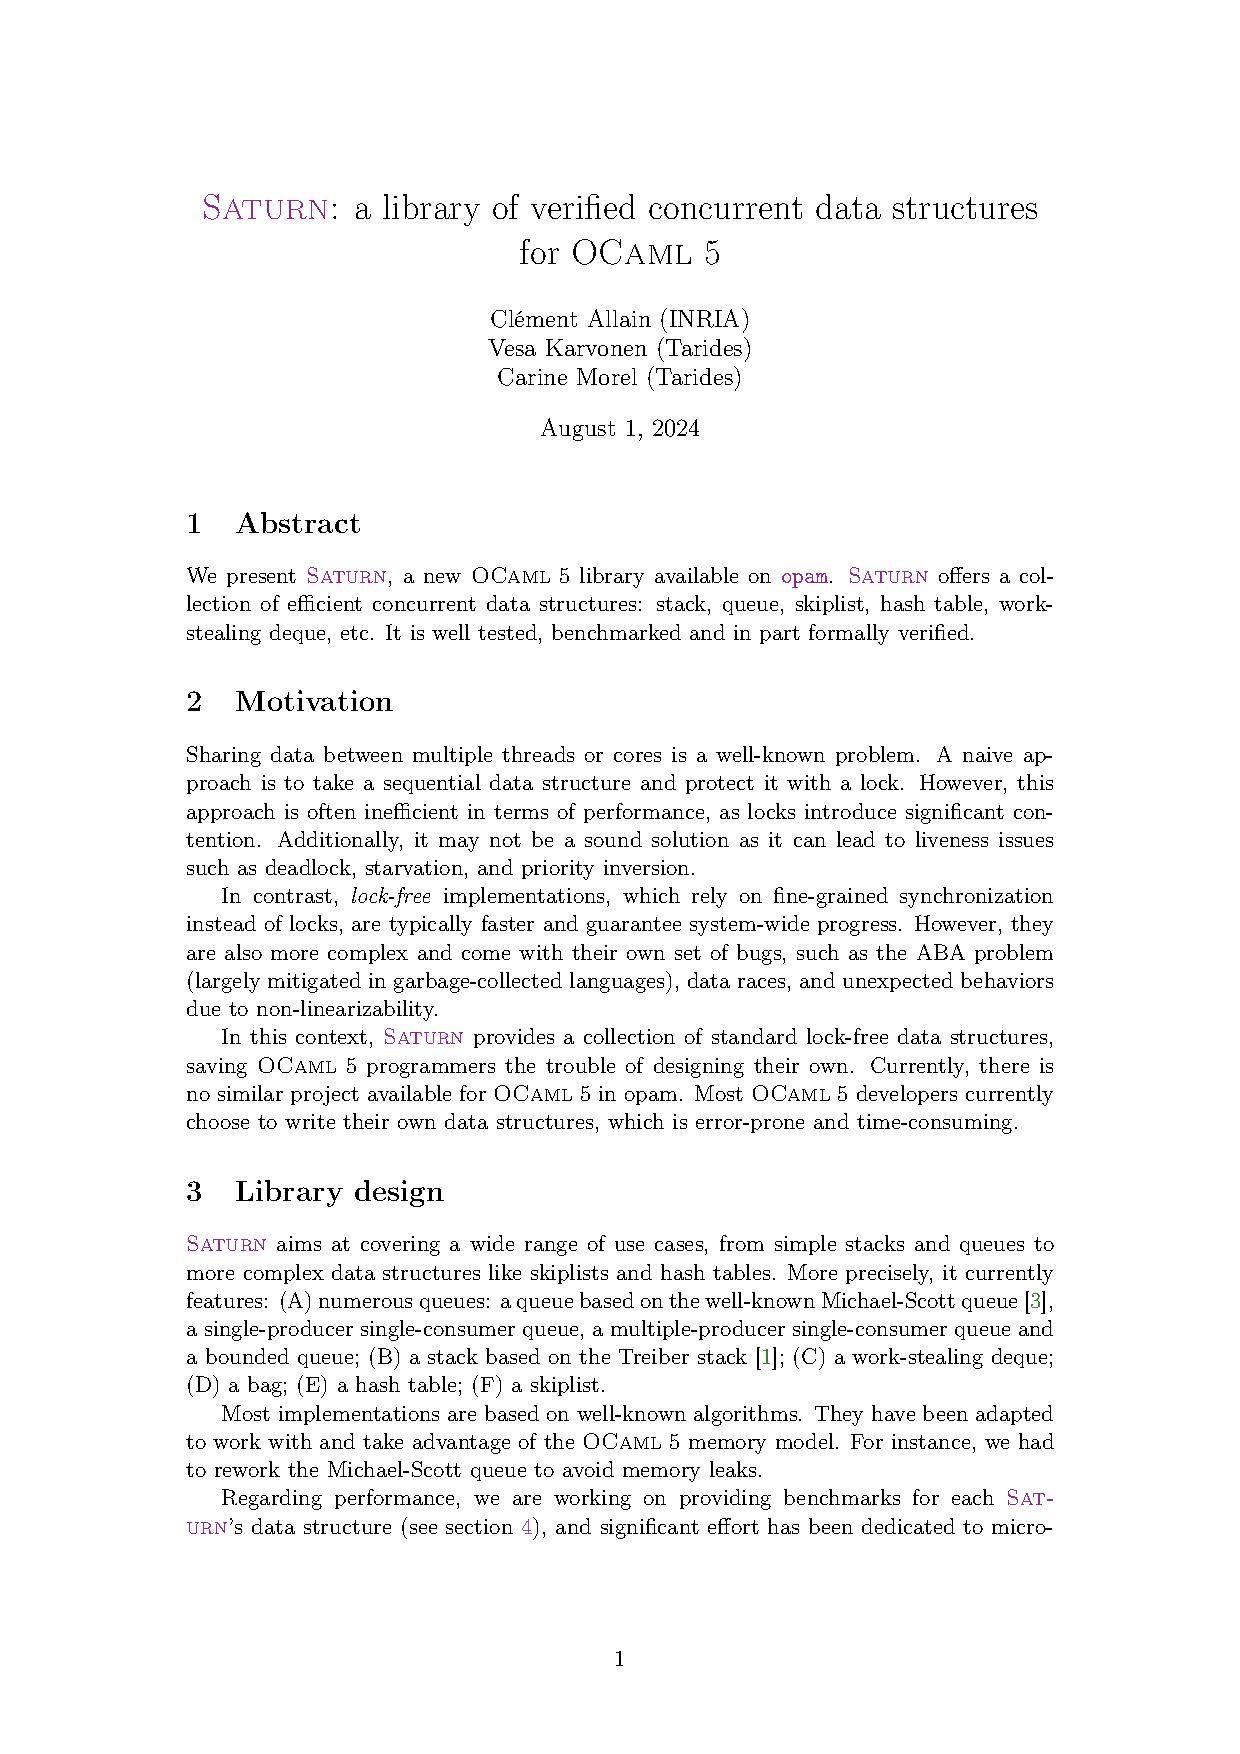
\includegraphics[scale=0.5]{images/allain-karvonen-morel-24.pdf}
\end{frame}

% ---------------------------------------------------------

\begin{frame}{\OCaml vers \Zoo}
\centering
\Huge
\begin{tabular}{ccccc}
      \begin{tabular}{c}
          
\includegraphics[scale=0.25]{images/ocaml.png}
        \\
          
\includegraphics[scale=0.1]{images/dune.png}
      \end{tabular}
    &&
      $\stackrel{\mbox{\Large\texttt{ocaml2zoo}}}{\longrightarrow}$
    &&
      \begin{tabular}{c}
          
\includegraphics[scale=0.4]{images/coq.png}
        \\
          \textcolor{Green}{\Zoo}
        \\\\
          
\includegraphics[scale=0.5]{images/iris.png}
      \end{tabular}
\end{tabular}
\end{frame}

% ---------------------------------------------------------

\begin{frame}[fragile]{\texttt{Store} : deux interfaces}
\centering
\footnotesize
\begin{minted}{ocaml}
          type t
          type store = t
          val create : unit -> t
          module Ref : sig
            type 'a t
            val make : store -> 'a -> 'a t
            val get : store -> 'a t -> 'a
            val set : store -> 'a t -> 'a -> unit
          end
\end{minted}
\vfill
\begin{minipage}[t]{.49\textwidth}
\begin{minted}{ocaml}
type snapshot
val capture :
  store -> snapshot
val restore :
  store -> snapshot -> unit
\end{minted}
\end{minipage}
\hfill
\begin{minipage}[t]{.49\textwidth}
\begin{minted}{ocaml}
type transaction
val transaction :
  store -> transaction
val rollback :
  store -> transaction -> unit
val commit :
  store -> transaction -> unit
\end{minted}
\end{minipage}
\end{frame}

% ---------------------------------------------------------

\begin{frame}[fragile]{\texttt{ocaml2zoo} appliqué à \texttt{Store}}
\centering
\scriptsize
\hspace{-6mm}
\begin{minipage}[t]{.45\textwidth}
\begin{minted}{ocaml}
let restore t s =
  if t != s.snap_store then (
    assert false
  ) else (
    let root = s.snap_root in
    match !root with
    | Root ->
        ()
    | Diff _ ->
        reroot root ;
        t.gen <- s.snap_gen + 1 ;
        t.root <- root
  )
\end{minted}
\end{minipage}
\hfill
\begin{minipage}[t]{.55\textwidth}
\begin{minted}{coq}
Definition pstore_restore : val :=
  fun: "t" "s" =>
    if: "t" != "s".<snap_store> then (
      Fail
    ) else (
      let: "root" := "s".<snap_root> in
      match: !"root" with
      | Root =>
          ()
      | Diff <> <> <> <> =>
          pstore_reroot "root" ;;
          "t" <-{gen} "s".<snap_gen> + #1 ;;
          "t" <-{root} "root"
      end
    ).
\end{minted}
\end{minipage}
\end{frame}

% ---------------------------------------------------------

\begin{frame}{Spécification : un simple état mutable\dots}
\large
\[
  \iSpec{
    \iTrue
  }{
    \texttt{create ()}
  }{
    t
  }{
    \textcolor{red}{\mathrm{store}}\ t\ \emptyset
  }
\]
\vfill
\[
  \iSpec{
    \textcolor{red}{\mathrm{store}}\ t\ \sigma
  }{
    \texttt{ref}\ t\ v
  }{
    r
  }{
    r \notin \dom{\sigma} \iSep
    \textcolor{red}{\mathrm{store}}\ t\ \sigma[r \mapsto v]
  }
\]
\vfill
\[
  \begin{array}{cccc}
      \iSpec{
        \textcolor{red}{\mathrm{store}}\ t\ \sigma \iSep
        \sigma (r) = v
      }{
        \texttt{get}\ t\ r
      }{
        v
      }{
        \textcolor{red}{\mathrm{store}}\ t\ \sigma
      }
    &&&
      \iSpec{
        \textcolor{red}{\mathrm{store}}\ t\ \sigma \iSep
        r \in \dom{\sigma}
      }{
        \texttt{set}\ t\ r\ v
      }{
        v
      }{
        \textcolor{red}{\mathrm{store}}\ t\ \sigma[r \mapsto v]
      }
  \end{array}
\]
\end{frame}

% ---------------------------------------------------------

\begin{frame}{\dots avec des versions persistantes}
\Large
\[
  \iSpec{
    \textcolor{red}{\mathrm{store}}\ t\ \sigma
  }{
    \texttt{capture}\ t
  }{
    s
  }{
    \textcolor{red}{\mathrm{store}}\ t\ \sigma \iSep
    \textcolor{olive}{\mathrm{snapshot}}\ t\ s\ \sigma
  }
\]
\vfill
\[
  \iSpec{
    \textcolor{red}{\mathrm{store}}\ t\ \sigma \iSep
    \textcolor{olive}{\mathrm{snapshot}}\ t\ s\ \sigma'
  }{
    \texttt{restore}\ t\ s
  }{
    \texttt{()}
  }{
    \textcolor{red}{\mathrm{store}}\ t\ \sigma'
  }
\]
\end{frame}

% ---------------------------------------------------------

\begin{frame}[plain, noframenumbering]
\LARGE
\begin{center}
  Merci de votre attention!
\end{center}
\end{frame}

% ---------------------------------------------------------

\appendix

% ---------------------------------------------------------

\begin{frame}{Implementation \emph{without} elision}
\centering
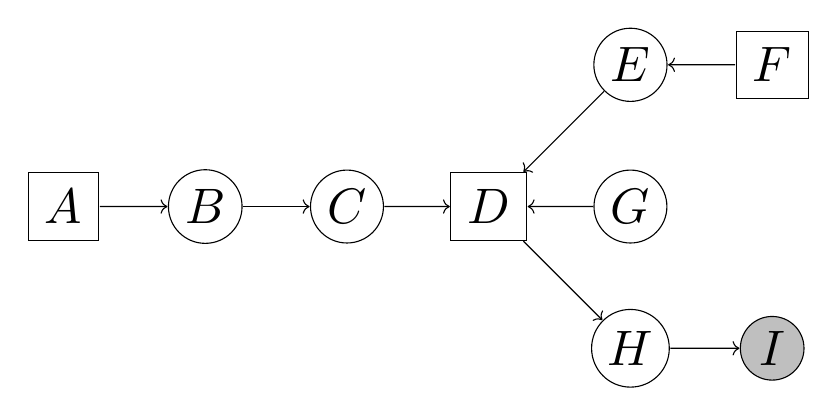
\begin{tikzpicture}[scale=1.8, every node/.style={transform shape}]
  \node [cnode] (a) at (0,0) {$A$} ;
  \node [node] (b) at (1,0) {$B$} ;
  \node [node] (c) at (2,0) {$C$} ;
  \node [cnode] (d) at (3,0) {$D$} ;
  \node [node] (e) at (4,1) {$E$} ;
  \node [cnode] (f) at (5,1) {$F$} ;
  \node [node] (g) at (4,0) {$G$} ;
  \node [node] (h) at (4,-1) {$H$} ;
  \node [node, root] (i) at (5,-1) {$I$} ;
  
  \graph {
    (a) -> (b) -> (c) -> (d) -> (h) -> (i) ;
    (d) <- (e) <- (f) ;
    (d) <- (g) ;
  } ;
\end{tikzpicture}
\end{frame}

% ---------------------------------------------------------

\begin{frame}{Rerooting \emph{without} elision}
\centering
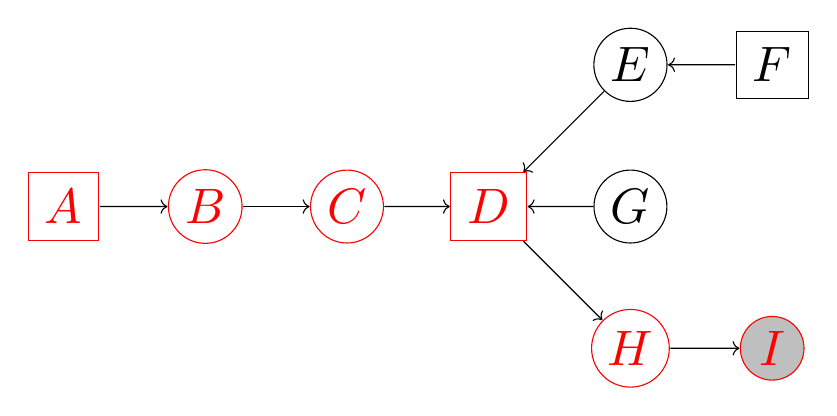
\begin{tikzpicture}[scale=1.8, every node/.style={transform shape}]
  \node [cnode, red] (a) at (0,0) {$A$} ;
  \node [node, red] (b) at (1,0) {$B$} ;
  \node [node, red] (c) at (2,0) {$C$} ;
  \node [cnode, red] (d) at (3,0) {$D$} ;
  \node [node] (e) at (4,1) {$E$} ;
  \node [cnode] (f) at (5,1) {$F$} ;
  \node [node] (g) at (4,0) {$G$} ;
  \node [node, red] (h) at (4,-1) {$H$} ;
  \node [node, red, root] (i) at (5,-1) {$I$} ;
  
  \graph {
    (a) -> (b) -> (c) -> (d) -> (h) -> (i) ;
    (d) <- (e) <- (f) ;
    (d) <- (g) ;
  } ;
\end{tikzpicture}
\end{frame}

% ---------------------------------------------------------

\begin{frame}{Rerooting \emph{without} elision}
\centering
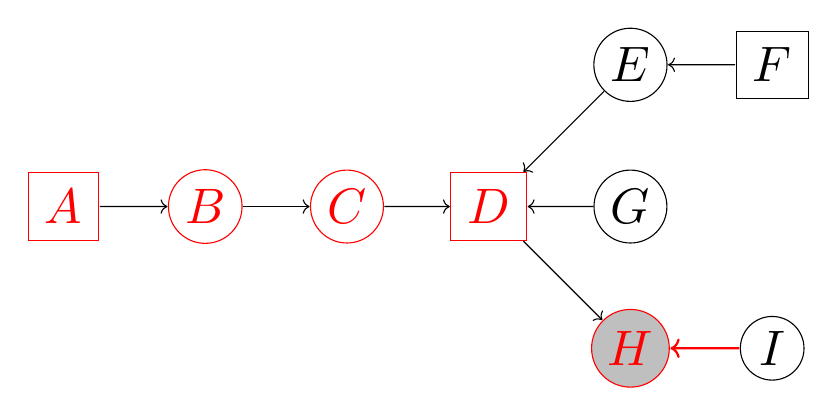
\begin{tikzpicture}[scale=1.8, every node/.style={transform shape}]
  \node [cnode, red] (a) at (0,0) {$A$} ;
  \node [node, red] (b) at (1,0) {$B$} ;
  \node [node, red] (c) at (2,0) {$C$} ;
  \node [cnode, red] (d) at (3,0) {$D$} ;
  \node [node] (e) at (4,1) {$E$} ;
  \node [cnode] (f) at (5,1) {$F$} ;
  \node [node] (g) at (4,0) {$G$} ;
  \node [node, red, root] (h) at (4,-1) {$H$} ;
  \node [node] (i) at (5,-1) {$I$} ;
  
  \graph {
    (a) -> (b) -> (c) -> (d) -> (h) <-[red,thick] (i) ;
    (d) <- (e) <- (f) ;
    (d) <- (g) ;
  } ;
\end{tikzpicture}
\end{frame}

% ---------------------------------------------------------

\begin{frame}{Rerooting \emph{without} elision}
\centering
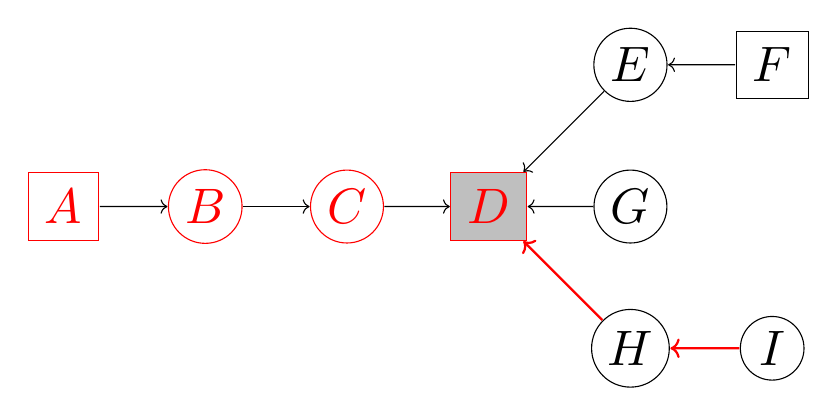
\begin{tikzpicture}[scale=1.8, every node/.style={transform shape}]
  \node [cnode, red] (a) at (0,0) {$A$} ;
  \node [node, red] (b) at (1,0) {$B$} ;
  \node [node, red] (c) at (2,0) {$C$} ;
  \node [cnode, red, root] (d) at (3,0) {$D$} ;
  \node [node] (e) at (4,1) {$E$} ;
  \node [cnode] (f) at (5,1) {$F$} ;
  \node [node] (g) at (4,0) {$G$} ;
  \node [node] (h) at (4,-1) {$H$} ;
  \node [node] (i) at (5,-1) {$I$} ;
  
  \graph {
    (a) -> (b) -> (c) -> (d) ;
    { [edges={red,thick}] (d) <- (h) <- (i) } ;
    (d) <- (e) <- (f) ;
    (d) <- (g) ;
  } ;
\end{tikzpicture}
\end{frame}

% ---------------------------------------------------------

\begin{frame}{Rerooting \emph{without} elision}
\centering
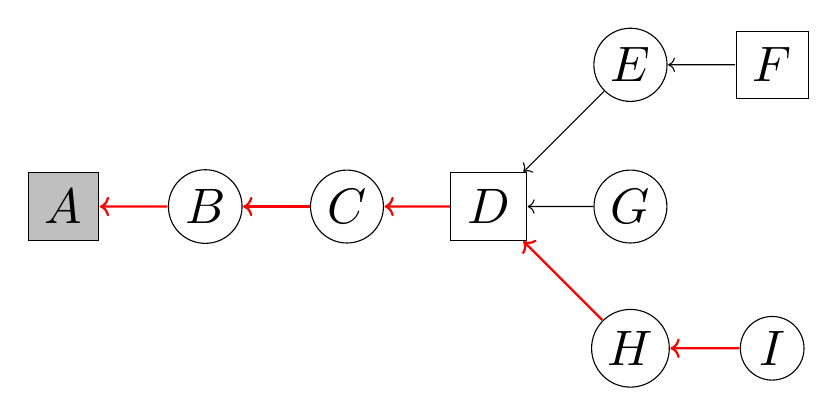
\begin{tikzpicture}[scale=1.8, every node/.style={transform shape}]
  \node [cnode, root] (a) at (0,0) {$A$} ;
  \node [node] (b) at (1,0) {$B$} ;
  \node [node] (c) at (2,0) {$C$} ;
  \node [cnode] (d) at (3,0) {$D$} ;
  \node [node] (e) at (4,1) {$E$} ;
  \node [cnode] (f) at (5,1) {$F$} ;
  \node [node] (g) at (4,0) {$G$} ;
  \node [node] (h) at (4,-1) {$H$} ;
  \node [node] (i) at (5,-1) {$I$} ;
  
  \graph {
    { [edges={red,thick}] (a) <- (b) <- (c) <- (d) <- (h) <- (i) } ;
    (d) <- (e) <- (f) ;
    (d) <- (g) ;
  } ;
\end{tikzpicture}
\end{frame}

% ---------------------------------------------------------

\begin{frame}{Historical tree \& generations}
\centering
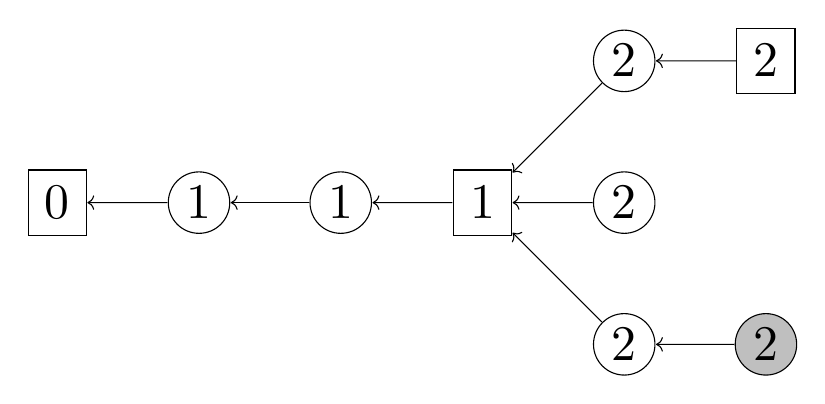
\begin{tikzpicture}[scale=1.8, every node/.style={transform shape}]
  \node [cnode] (a) at (0,0) {$0$} ;
  \node [node] (b) at (1,0) {$1$} ;
  \node [node] (c) at (2,0) {$1$} ;
  \node [cnode] (d) at (3,0) {$1$} ;
  \node [node] (e) at (4,1) {$2$} ;
  \node [cnode] (f) at (5,1) {$2$} ;
  \node [node] (g) at (4,0) {$2$} ;
  \node [node] (h) at (4,-1) {$2$} ;
  \node [node, root] (i) at (5,-1) {$2$} ;
  
  \graph {
    (a) <- (b) <- (c) <- (d) <- (h) <- (i) ;
    (d) <- (e) <- (f) ;
    (d) <- (g) ;
  } ;
\end{tikzpicture}
\end{frame}

% ---------------------------------------------------------

\begin{frame}{Implementation \emph{with} elision}
\centering
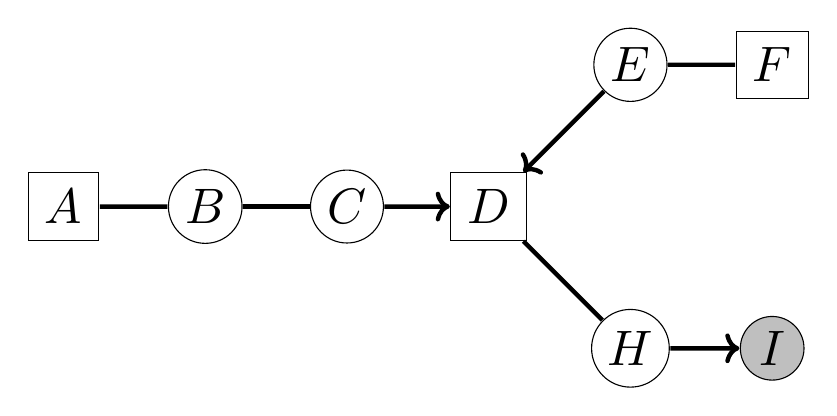
\begin{tikzpicture}[scale=1.8, every node/.style={transform shape}]
  \node [cnode] (a) at (0,0) {$A$} ;
  \node [node] (b) at (1,0) {$B$} ;
  \node [node] (c) at (2,0) {$C$} ;
  \node [cnode] (d) at (3,0) {$D$} ;
  \node [node] (e) at (4,1) {$E$} ;
  \node [cnode] (f) at (5,1) {$F$} ;
  \node [node] (h) at (4,-1) {$H$} ;
  \node [node, root] (i) at (5,-1) {$I$} ;
  
  \graph [edges=ultra thick] {
    (a) -- (b) -- (c) -> (d) -- (h) -> (i) ;
    (d) <- (e) -- (f) ;
  } ;
\end{tikzpicture}
\end{frame}

% ---------------------------------------------------------

\begin{frame}{Rerooting \emph{with} elision}
\centering
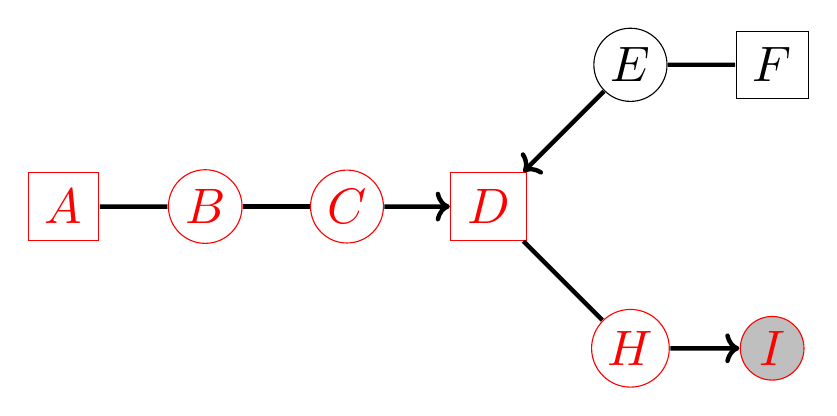
\begin{tikzpicture}[scale=1.8, every node/.style={transform shape}]
  \node [cnode, red] (a) at (0,0) {$A$} ;
  \node [node, red] (b) at (1,0) {$B$} ;
  \node [node, red] (c) at (2,0) {$C$} ;
  \node [cnode, red] (d) at (3,0) {$D$} ;
  \node [node] (e) at (4,1) {$E$} ;
  \node [cnode] (f) at (5,1) {$F$} ;
  \node [node, red] (h) at (4,-1) {$H$} ;
  \node [node, red, root] (i) at (5,-1) {$I$} ;
  
  \graph [edges=ultra thick] {
    (a) -- (b) -- (c) -> (d) -- (h) -> (i) ;
    (d) <- (e) -- (f) ;
  } ;
\end{tikzpicture}
\end{frame}

% ---------------------------------------------------------

\begin{frame}{Rerooting \emph{with} elision}
\centering
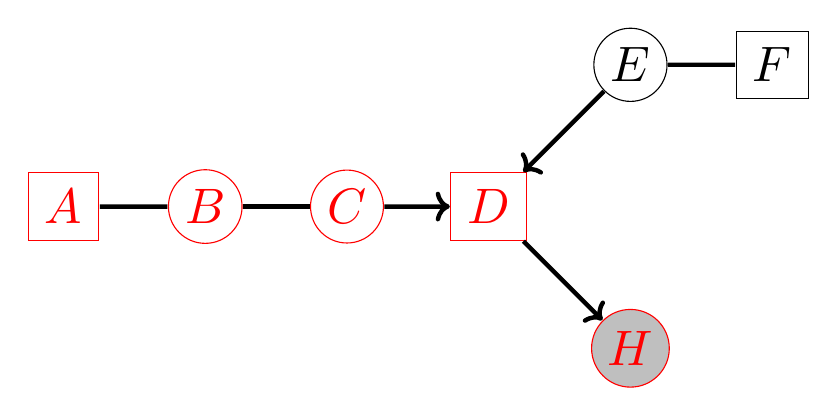
\begin{tikzpicture}[scale=1.8, every node/.style={transform shape}]
  \node [cnode, red] (a) at (0,0) {$A$} ;
  \node [node, red] (b) at (1,0) {$B$} ;
  \node [node, red] (c) at (2,0) {$C$} ;
  \node [cnode, red] (d) at (3,0) {$D$} ;
  \node [node] (e) at (4,1) {$E$} ;
  \node [cnode] (f) at (5,1) {$F$} ;
  \node [node, red, root] (h) at (4,-1) {$H$} ;
  
  \graph [edges=ultra thick] {
    (a) -- (b) -- (c) -> (d) -> (h) ;
    (d) <- (e) -- (f) ;
  } ;
\end{tikzpicture}
\end{frame}

% ---------------------------------------------------------

\begin{frame}{Rerooting \emph{with} elision}
\centering
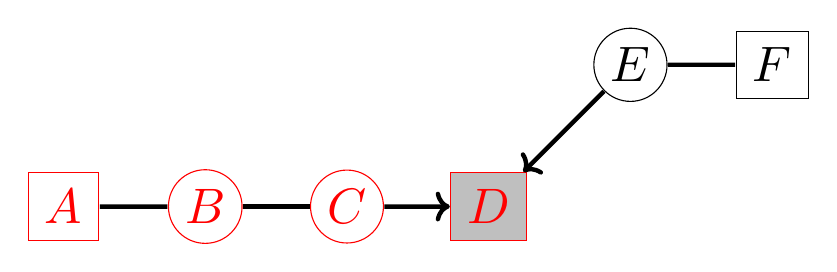
\begin{tikzpicture}[scale=1.8, every node/.style={transform shape}]
  \node [cnode, red] (a) at (0,0) {$A$} ;
  \node [node, red] (b) at (1,0) {$B$} ;
  \node [node, red] (c) at (2,0) {$C$} ;
  \node [cnode, red, root] (d) at (3,0) {$D$} ;
  \node [node] (e) at (4,1) {$E$} ;
  \node [cnode] (f) at (5,1) {$F$} ;
  
  \graph [edges=ultra thick] {
    (a) -- (b) -- (c) -> (d) ;
    (d) <- (e) -- (f) ;
  } ;
\end{tikzpicture}
\end{frame}

% ---------------------------------------------------------

\begin{frame}{Rerooting \emph{with} elision}
\centering
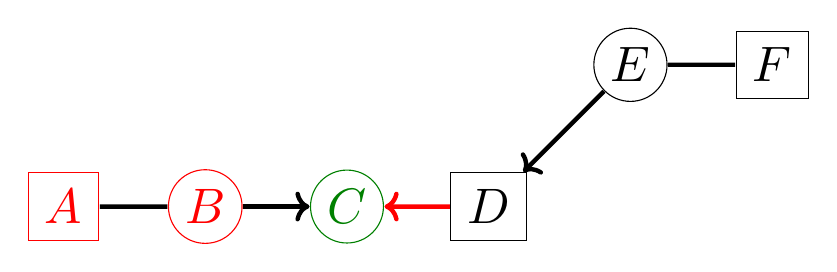
\begin{tikzpicture}[scale=1.8, every node/.style={transform shape}]
  \node [cnode, red] (a) at (0,0) {$A$} ;
  \node [node, red] (b) at (1,0) {$B$} ;
  \node [node, Green] (c) at (2,0) {$C$} ;
  \node [cnode] (d) at (3,0) {$D$} ;
  \node [node] (e) at (4,1) {$E$} ;
  \node [cnode] (f) at (5,1) {$F$} ;
  
  \graph [edges=ultra thick] {
    (a) -- (b) -> (c) <-[red] (d) ;
    (d) <- (e) -- (f) ;
  } ;
\end{tikzpicture}
\end{frame}

% ---------------------------------------------------------

\begin{frame}{Rerooting \emph{with} elision}
\centering
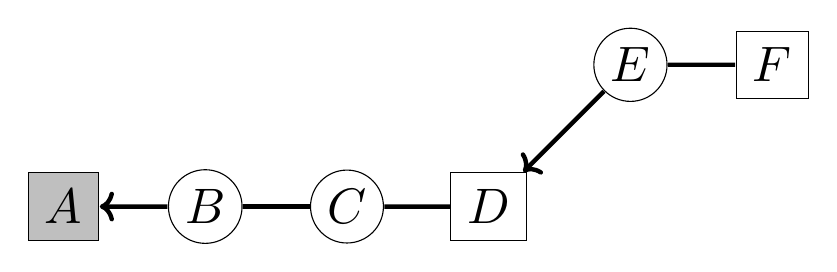
\begin{tikzpicture}[scale=1.8, every node/.style={transform shape}]
  \node [cnode, root] (a) at (0,0) {$A$} ;
  \node [node] (b) at (1,0) {$B$} ;
  \node [node] (c) at (2,0) {$C$} ;
  \node [cnode] (d) at (3,0) {$D$} ;
  \node [node] (e) at (4,1) {$E$} ;
  \node [cnode] (f) at (5,1) {$F$} ;
  
  \graph [edges=ultra thick] {
    (a) <- (b) -- (c) -- (d) ;
    (d) <- (e) -- (f) ;
  } ;
\end{tikzpicture}
\end{frame}

% ---------------------------------------------------------

\end{document}
